\section{Initial Value Problems for ODEs}
\subsection{Problem 9.2}
\subsubsection*{Write each of the following ODEs as an equivalent first-order system of ODEs:}
$(a)$ Van der Pol Equation:
\begin{equation*}
y'' = y'\left(1-y^2\right)-y
\end{equation*}
\textbf{Solution.} Define a new vector $\mathbf{U}$ such that
\begin{align*}
\mathbf{U} = 
\begin{bmatrix}
u_1\\
u_2\\
\end{bmatrix}
=
\begin{bmatrix}
y\\
y'\\
\end{bmatrix}\\
\mathbf{U'} =
\begin{bmatrix}
u_1'\\
u_2'\\
\end{bmatrix} =
\begin{bmatrix}
y'\\
y''\\
\end{bmatrix}\\
\end{align*}
So that we can have
\begin{equation*}\boxed{
\begin{bmatrix}
u_1'\\
u_2'\\
\end{bmatrix} =
\begin{bmatrix}
u_2\\
u_2\left(1-u_1^2\right)-u_1\\
\end{bmatrix}}
\end{equation*}
\\
\\
$(b)$ Blasius equation:
\begin{equation*}
y''' = -yy''
\end{equation*}
\textbf{Solution.} Define a new vector $\mathbf{U}$ such that
\begin{align*}
\mathbf{U} = 
\begin{bmatrix}
u_1\\
u_2\\
u_3\\
\end{bmatrix}
=
\begin{bmatrix}
y\\
y'\\
y''\\
\end{bmatrix}\\
\mathbf{U'} =
\begin{bmatrix}
u_1'\\
u_2'\\
u_3'
\end{bmatrix} =
\begin{bmatrix}
y'\\
y''\\
y'''
\end{bmatrix}\\
\end{align*}
So that we can have
\begin{equation*}\boxed{
	\begin{bmatrix}
	u_1'\\
	u_2'\\
	u_3'
	\end{bmatrix} =
	\begin{bmatrix}
	u_2\\
	u_3\\
	-u_1u_3
	\end{bmatrix}}
\end{equation*}
\\
\\
$(c)$ Newton's Second Law of Motion for two-body problem:
\begin{align*}
y_1'' &= -GMy_1/\left(y_1^2+y_2^2\right)^{3/2}\\
y_2'' &= -GMy_2/\left(y_1^2+y_2^2\right)^{3/2}
\end{align*}

\textbf{Solution.} Define a new vector $\mathbf{U}$ such that
\begin{align*}
\mathbf{U} = 
\begin{bmatrix}
u_1\\
u_2\\
u_3\\
u_4
\end{bmatrix}
=
\begin{bmatrix}
y_1\\
y_1'\\
y_2\\
y_2'
\end{bmatrix}\\
\mathbf{U'} =
\begin{bmatrix}
u_1'\\
u_2'\\
u_3'\\
u_4'
\end{bmatrix} =
\begin{bmatrix}
y_1'\\
y_1''\\
y_2'\\
y_2''
\end{bmatrix}\\
\end{align*}
So that we can have
\begin{equation*}\boxed{
	\begin{bmatrix}
	u_1'\\
	u_2'\\
	u_3'\\
	u_4'
	\end{bmatrix} =
	\begin{bmatrix}
	u_2\\
	-GMu_1/\left(u_1^2+u_3^2\right)^{3/2}\\
	u_4\\
	-GMu_3/\left(u_1^2+u_3^2\right)^{3/2}\\
	\end{bmatrix}}
\end{equation*}

\subsection{Problem 9.4}
\textbf{Consider the ODE $y'=-5y$ with initial condition $y(0) = 1$. We will solve this ODE numerically using a step size of $h=0.5$.}
\subsubsection*{$(a)$ Are solutions to this ODE stable?}
\textbf{Solution.} Solving the ODE, we have
\begin{align*}
\frac{dy}{dt} &= -5y \\
\frac{dy}{y} &= -5\:dt \\
\int\frac{dy}{y} &= \int-5\:dt \\
\ln y &= -5t + C \\
y &= e^{-5t+C} \\
\end{align*}
Visualize the family of curves as solutions to this ODE.
\begin{figure}[H]
	\centering
	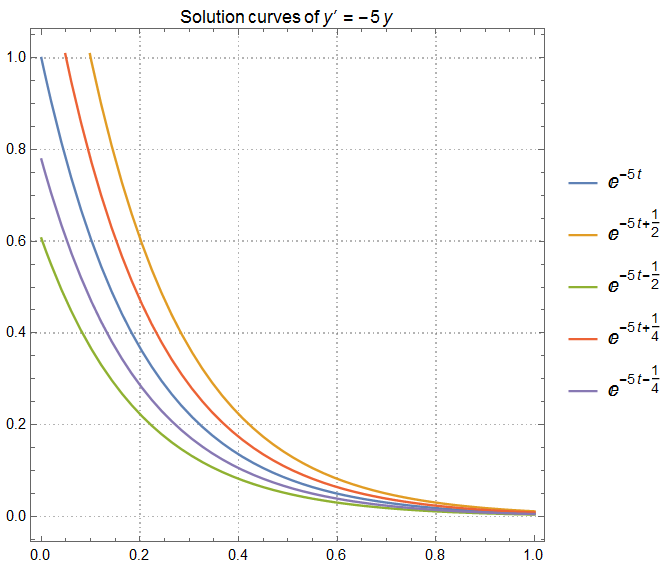
\includegraphics[width=\textwidth]{family}
\end{figure}
Applying the initial condition, we have $y = e^{-5t}$, which is shown in blue. If the initial value is perturbed, then the perturbed solution remains close to the original solution. Moreover, notice that the solution curves $\mathbf{y} \rightarrow 0$ as $t \rightarrow \infty$. Therefore, solutions to this ODE are asymptotically stable.

\subsubsection*{$(b)$ Is Euler's method stable for this ODE using this step size?}
\textbf{Solution.} In order for Euler's method to be stable in the ODE $y' = \lambda y$, the step size $h$ must satisfy the inequality
\begin{align*}
\left|1+h\lambda\right| &\leq 1\\
\left|1+(0.5)(-5)\right| &\leq 1\\
\left|1-2.5\right| &\leq 1\\
\Aboxed{1.5 \not\leq 1}
\end{align*}
It turns out that the Euler's method is not stable for the ODE given above.

\subsubsection*{$(c)$ Compute the numerical value for the approximate solution at $t=0.5$ given by Euler's method.}
\textbf{Solution.} Euler's explicit method is given by
\begin{align*}
y_{k+1} &= y_k + h_kf(t_k,y_k)\\
y_1 &= y_0 + (0.5)(-5y_0)\\
y_1 &= 1 + (0.5)(-5\cdot 1)\\
\Aboxed{y_1 &= -1.5}
\end{align*}

\subsubsection*{$(b)$ Is the backward Euler method stable for this ODE using this step size?}
\textbf{Solution.} For the backward Euler method to be stable we must have
\begin{align*}
\left|\frac{1}{1-h\lambda}\right| &\leq 1\\
\left|\frac{1}{1-(0.5)(-5)}\right| &\leq 1\\
\left|\frac{1}{-1.5}\right| &\leq 1\\
\Aboxed{0.\bar{6} \leq 1}
\end{align*}
Actually, this inequality holds for any $h>0$ when $\text{Re}(\lambda)<0$. Therefore, the backward Euler method is stable for this ODE.

\subsubsection*{$(c)$ Compute the numerical value for the approximate solution at $t=0.5$ given by the backward Euler method.}
\textbf{Solution.} The backward Euler method is given by
\begin{align*}
y_{k+1} &= y_k + h_kf(t_{k+1},y_{k+1})\\
y_1 &= y_0 + (0.5)(-5y_1)\\
y_1 &= 1 - 2.5y_1\\
3.5y_1 &= 1\\
\Aboxed{y_1 &= 0.285714\ldots}
\end{align*}

\subsection{Problem 9.8}
\textbf{Consider the IVP for the ODE $y'=-y^2$ with the initial condition $y(0)=1$. We will use the backward Euler method to compute the approximate value of the solution $y_1$ at time $t_1$=0.1 (i.e. taking one step using the backward Euler method with step size $h=0.1$ starting from $y_0=1$ at $t_0=0$). Since the backward Euler method is implicit, and the ODE is nonlinear, we will need to solve a nonlinear algebraic equation for $y_1$.}
\subsubsection*{$(a)$ Write out that nonlinear algebraic equation for $y_1$.}
\textbf{Solution.} The backward Euler method is given by
\begin{align*}
y_{k+1} &= y_k + h_kf(t_{k+1},y_{k+1})\\
y_1 &= 1 + (0.1)(-y_1^2)\\
\end{align*}
\begin{equation}\label{quad}
\boxed{(0.1)y_1^2 + y_1 - 1 = 0}\\
\end{equation}

\subsubsection*{$(b)$ Write out Newton iteration for solving the nonlinear algebraic equation.}
\textbf{Solution.} The Newton's root-finding method is given by
\begin{align*}
y^* &= y - \frac{f(y)}{f'(y)}\\
f(y) &= (0.1)y^2 + y - 1\\
f'(y) &= (0.2)y+1\\
\Aboxed{y^* &= y - \frac{(0.1)y^2+y-1}{(0.2)y+1}}
\end{align*}

\subsubsection*{$(c)$ Obtain a starting guess for the Newton iteration by using one step of Euler's method for the ODE.}
\textbf{Solution.} Euler's explicit method is given by
\begin{align*}
y_{k+1} &= y_k + h_kf(t_k,y_k)\\
y_1 &= 1 + (0.1)(-y_0^2)\\
y_1 &= 1 + (0.1)(-1^2)\\
\Aboxed{y_1 &= 0.9}
\end{align*}

\subsubsection*{$(d)$ Finally, compute an approximate value for the solution $y_1$ by using one iteration of Newton's method for the nonlinear algebraic equation.}
\textbf{Solution.} Let's have one iteration:
\begin{align*}
y^* &= y - \frac{\frac{1}{10}y^2+y-1}{\frac{1}{5}y+1}\\
y^* &= 0.9 - \frac{(0.1)(0.9)^2 + (0.9) - 1}{(0.2)(0.9)+1}\\
y^* &= 0.9 - \frac{-0.019}{1.18}\\
y^* &= 0.9 + 0.0161017\\
\Aboxed{y^* &= 0.9161017}
\end{align*}

\subsubsection*{Further Notes.} Solving the nonlinear equation (\ref{quad}) analytically, we have
\begin{align*}
(0.1)&y^2 + y - 1 = 0\\
y &= \frac{-1 \pm \sqrt{1^2 - 4(0.1)(-1)}}{0.2}\\
y &= \frac{-1 \pm \sqrt{1.4}}{0.2}\\
\Aboxed{y_1 &= 0.9160797\cdots}\\
y_2 &= -10.9160797\cdots
\end{align*}
Notice that $y^*$ is already close to the true value given in $y_1$ above.

\subsection{Problem 9.9}
\textbf{For each property listed below, state which of the following three ODE methods has or have the given property.}
\begin{align*}
(1)\:y_{k+1} &= y_k + \frac{h}{2}\left(f(t_k, y_k) + f\left(t_{k+1},y_k+hf\left(t_k, y_k\right)\right)\right)\\
& \Aboxed{a, d, f}\\
(2)\:y_{k+1} &= y_k + \frac{h}{2}\left(3f(t_k, y_k) - f(t_{k-1}, y_{k-1})\right)\\
& \Aboxed{a}\\
(3)\:y_{k+1} &= y_k + \frac{h}{2}\left(f(t_k, y_k) + f(t_{k+1}, y_{k+1})\right)\\
& \Aboxed{a, d, e, c, g}\\
\end{align*}